
\documentclass{article}

\usepackage[a4paper, left=1.5cm, right=1.5cm, top=2cm, bottom=2cm]{geometry}
\usepackage{../../../../components/components}

\usepackage{fancyhdr}


\usepackage{tikz}
\usepackage{pgfplots}
\usepackage{hyperref}
\pgfplotsset{compat=1.18}
\usetikzlibrary{arrows.meta, calc}
% Configuration des en-têtes et pieds de page
\pagestyle{fancy}
\fancyhf{} % reset tout

\fancyhead[L]{Préparation CAPES}
\fancyhead[C]{Analyse}
\fancyhead[R]{2025-2026}

\fancyfoot[L]{Ewen Rodrigues de Oliveira}
\fancyfoot[R]{\thepage}

\begin{document}

\docTitle{Chapitre 5 : Intégration}

\noindent Ce cours reprend les notions d'intégration \textit{(au sens de Riemann)} vues en terminale et en première année de licence. Il s'agit de voir, une bonne fois pour toutes, la théorie et les outils nécessaires au calcul d'intégrales.



\section{Introduction et motivation géométrique}

La théorie de l'intégration cherche à répondre à un problème fondamental de la géométrie plane : comment mesurer l'aire d'un domaine délimité par des courbes non rectilignes ?\\

Historiquement, la méthode d'épuisement d'Archimède consistait à approcher l'aire sous une courbe par des polygones inscrits ou circonscrits. Au XVIIe siècle, Riemann formalise cette intuition à l'aide de fonctions simples particulières : les fonctions en escalier.

\illustration{Considérons la fonction carré $f(x) = x^2$ sur le segment $[0, 1]$. On souhaite évaluer l'aire $\mathcal{A}$ sous sa courbe. Pour cela, on subdivise l'intervalle $[0,1]$ en $n$ sous-intervalles égaux de longueur $\frac{1}{n}$. On définit alors deux sommes d'aires de rectangles (les rectangles inférieurs d'aire globale $I_n$ et supérieurs d'aire globale $S_n$) :
$$I_n = \sum_{k=0}^{n-1} \frac{1}{n} \left(\frac{k}{n}\right)^2 = \frac{(n-1)n(2n-1)}{6n^3} = \frac{(n-1)(2n-1)}{6n^2}$$
$$S_n = \sum_{k=1}^{n} \frac{1}{n} \left(\frac{k}{n}\right)^2 = \frac{n(n+1)(2n+1)}{6n^3} = \frac{(n+1)(2n+1)}{6n^2}$$
On vérifie sans peine que pour tout $n \ge 1$ :
$$I_n \le \mathcal{A} \le S_n$$
Puisque $\lim_{n \to +\infty} I_n = \lim_{n \to +\infty} S_n = \frac{1}{3}$, d'après le théorème des gendarmes, l'aire sous la courbe de la fonction carré vaut précisément $\mathcal{A} = \frac{1}{3}$ u.a. (unités d'aire).}

\begin{center}
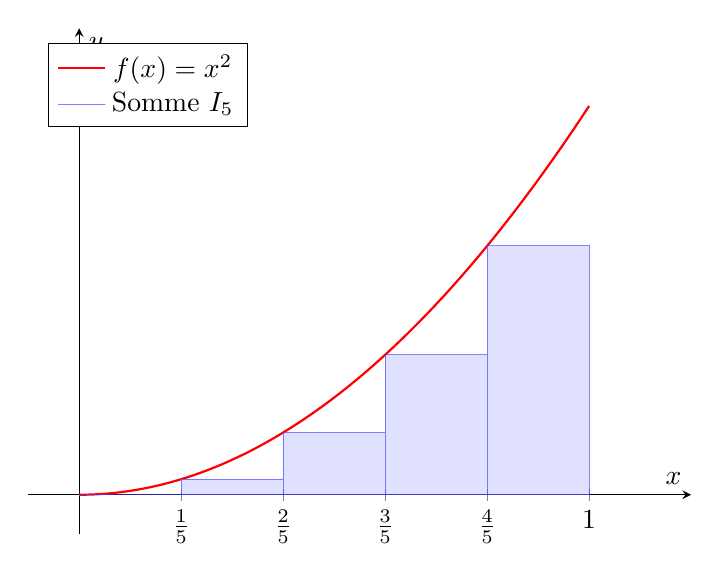
\begin{tikzpicture}
\begin{axis}[
    axis lines = middle,
    xlabel = $x$,
    ylabel = $y$,
    xmin = -0.1, xmax = 1.2,
    ymin = -0.1, ymax = 1.2,
    xtick = {0, 0.2, 0.4, 0.6, 0.8, 1.0},
    xticklabels = {0, $\frac{1}{5}$, $\frac{2}{5}$, $\frac{3}{5}$, $\frac{4}{5}$, 1},
    ytick = {0, 1},
    legend pos = north west,
    width = 10cm,
    height = 8cm
]
% Courbe f(x) = x^2
\addplot [
    domain=0:1, 
    samples=100, 
    color=red,
    thick
] {x^2};
\addlegendentry{$f(x)=x^2$}

% Rectangles inférieurs (n=5)
\addplot[ybar interval, fill=blue!20, draw=blue!80, opacity=0.6] coordinates {
(0, 0)
(0.2, 0.04)
(0.4, 0.16)
(0.6, 0.36)
(0.8, 0.64)
(1, 1)
};
\addlegendentry{Somme $I_5$}

\end{axis}
\end{tikzpicture}
\captionof{figure}{Approximation de l'aire sous la courbe par les rectangles inférieurs ($n=5$).}
\end{center}

\newpage

\section{Fonctions continues par morceaux}

La construction de l'intégrale rigoureuse au sens de Riemann s'appuie sur la notion de fonctions continues par morceaux, cadre standard d'étude de l'intégration.

\subsection{Subdivision d'un segment}

\definition{Soit $[a, b]$ un segment de $\mathbb{R}$ ($a < b$). On appelle \textbf{subdivision} de $[a, b]$ toute famille finie ordonnée de réels $\sigma = (x_i)_{0 \le i \le n}$ telle que :
$$a = x_0 < x_1 < x_2 < \dots < x_{n-1} < x_n = b$$
Le pas de la subdivision est défini par $p(\sigma) = \max_{0 \le i \le n-1} (x_{i+1} - x_i)$.\\
On dit d'une subdivision $\sigma'$ qu'elle est \textbf{plus fine} que $\sigma$ si $\sigma \subset \sigma'$ en tant qu'ensembles de points.}

\vocabulary{Une subdivision est dite \textbf{régulière} (ou \textbf{équirépartie}) si tous les intervalles de la subdivision possèdent la même longueur : pour tout $i \in \{0, \dots, n-1\}$, $x_{i+1} - x_i = \frac{b-a}{n}$.}

\subsection{Fonctions en escalier}

\definition{Soit $f : [a, b] \to \mathbb{R}$ une fonction.\\
On dit que $f$ est une \textbf{fonction en escalier} sur $[a, b]$ s'il existe une subdivision $\sigma = (x_i)_{0 \le i \le n}$ de $[a, b]$ telle que pour tout $i \in \{0, \dots, n-1\}$, la restriction de $f$ à l'intervalle ouvert $]x_i, x_{i+1}[$ est une fonction constante.\\
}

\vocabulary{On dit alors que la subdivision $\sigma$ est \textbf{adaptée} (ou \textbf{compatible}) à la fonction en escalier $f$.}

\attention{Une fonction en escalier n'est pas nécessairement constante aux points $x_i$ de la subdivision. Les valeurs de $f(x_i)$ aux nœuds n'altèrent en rien la nature de la fonction en escalier.}

\subsection{Fonctions continues par morceaux (CPM)}

La notion de continuité par morceaux généralise les fonctions en escalier en autorisant des variations non constantes entre les nœuds, afin de modéliser des fonctions plus complexes pour lesquelles l'intégration est encore possible.

\definition{Soit $f : [a, b] \to \mathbb{R}$ une fonction.\\
On dit que $f$ est \textbf{continue par morceaux} (CPM) sur $[a, b]$ s'il existe une subdivision $\sigma = (x_i)_{0 \le i \le n}$ de $[a, b]$ telle que :
\begin{enumerate}
    \item Pour tout $i \in \{0, \dots, n-1\}$, la restriction de $f$ à l'intervalle ouvert $]x_i, x_{i+1}[$ est continue.
    \item En chaque point de la subdivision $x_i$, $f$ admet une limite finie à gauche (si $i > 0$) et une limite finie à droite (si $i < n$).
\end{enumerate}}

\begin{center}
\begin{tikzpicture}
\begin{axis}[
    axis lines = middle,
    xlabel = $x$, ylabel = $y$,
    xmin = -0.5, xmax = 4.5,
    ymin = -0.5, ymax = 3.5,
    xtick = {0, 1.5, 3, 4},
    xticklabels = {$a=x_0$, $x_1$, $x_2$, $b=x_3$},
    ytick = \empty,
    width = 11cm, height = 6cm
]
% Tracé par morceaux d'une CPM
% Morceau 1 : [0, 1.5[
\addplot [domain=0:1.5, samples=50, blue, thick] {1 + 0.2*x^2};
\draw[blue, fill=blue] (axis cs:0, 1) circle (2pt);
\draw[blue, fill=white] (axis cs:1.5, 1.45) circle (2pt);

% Morceau 2 : [1.5, 3[
\addplot [domain=1.5:3, samples=50, blue, thick] {2.5 - 0.3*(x-2.2)^2};
\draw[blue, fill=blue] (axis cs:1.5, 2.35) circle (2pt);
\draw[blue, fill=white] (axis cs:3, 2.3) circle (2pt);

% Morceau 3 : [3, 4]
\addplot [domain=3:4, samples=50, blue, thick] {0.5 + 0.5*(x-3.5)};
\draw[blue, fill=blue] (axis cs:3, 1.0) circle (2pt);
\draw[blue, fill=blue] (axis cs:4, 0.75) circle (2pt);

\end{axis}
\end{tikzpicture}
\captionof{figure}{Graphe d'une fonction continue par morceaux sur $[a,b]$.}
\end{center}

\newpage

\theorem{Proposition}{Propriétés d'une fonction CPM}{false}{
    Soit $f : [a, b] \to \mathbb{R}$ continue par morceaux. Alors :
    \begin{enumerate}
        \item $f$ est \textbf{bornée} sur $[a, b]$ et atteint ses bornes (maximum et minimum) sur chaque intervalle ouvert $]x_i, x_{i+1}[$ prolongé à ses extrémités par les limites à gauche/droite.
        \item $f$ est continue par morceaux sur $[a,b]$ si et seulement s'il existe une fonction continue $g : [a,b] \to \mathbb{R}$ et une fonction en escalier $h : [a,b] \to \mathbb{R}$ telles que $f = g + h$.
    \end{enumerate}
}

\subsection{Primitives par morceaux}

\definition{Soit $f : [a, b] \to \mathbb{R}$ une fonction continue par morceaux. On appelle \textbf{primitive par morceaux} de $f$ sur $[a, b]$ toute fonction $F : [a, b] \to \mathbb{R}$ continue sur $[a, b]$ telle qu'il existe une subdivision $\sigma = (x_i)_{0 \le i \le n}$ adaptée à $f$ vérifiant :
\begin{enumerate}
    \item $F$ est dérivable sur chaque intervalle ouvert $]x_i, x_{i+1}[$ pour $0 \le i \le n-1$.
    \item Pour tout $x \in \bigcup_{i=0}^{n-1} ]x_i, x_{i+1}[$, $F'(x) = f(x)$.
\end{enumerate}}

\attention{Une primitive par morceaux $F$ de $f$ est obligatoirement \textbf{continue} sur le segment $[a, b]$ complet, bien que sa dérivée $F'$ puisse ne pas être définie aux points singuliers $x_i$.}

\theorem{Théorème}{Existence et structure des primitives par morceaux}{true}{
    Soit $f : [a, b] \to \mathbb{R}$ une fonction continue par morceaux.
    \begin{enumerate}
        \item $f$ admet au moins une primitive par morceaux $F$ sur $[a, b]$.
        \item Si $F$ et $G$ sont deux primitives par morceaux de $f$ sur $[a, b]$, alors il existe un réel $C$ tel que :
        $$\forall x \in [a, b], \quad F(x) - G(x) = C$$
    \end{enumerate}
}

\remark{Ce résultat montre que l'écart entre deux primitives par morceaux reste invariant sur tout le segment. C'est l'extension exacte de la propriété des primitives usuelles d'une fonction continue.}

\theorem{Proposition}{Lien entre signe de l'intégrande et sens de variation}{false}{
    Soit $f$ une fonction continue par morceaux sur $[a, b]$ et $F$ une primitive par morceaux de $f$.
    \begin{itemize}
        \item $F$ est croissante (resp. décroissante) sur $[a, b]$ si et seulement si $f \ge 0$ (resp. $f \le 0$) sauf éventuellement en un nombre fini de points.
        \item $F$ est constante sur $[a, b]$ si et seulement si $f = 0$ sauf éventuellement en un nombre fini de points.
    \end{itemize}
}

\training{Montrer la proposition précédente de manière rigoureuse.}
\noindent\carreaux{9}
\theorem{Corollaire}{Inégalité des accroissements finis par morceaux}{false}{
    Soit $f : [a, b] \to \mathbb{R}$ une fonction CPM et $F$ une primitive par morceaux de $f$.\\
    S'il existe deux réels $m$ et $M$ tels que pour tout $x \in [a, b]$ (sauf un nombre fini de points), $m \le f(x) \le M$, alors :
    $$m(b-a) \le F(b) - F(a) \le M(b-a)$$
}
\noindent{\textbf{Preuve :}\\
    Puisque $F$ est une primitive par morceaux de la fonction continue par morceaux $f$ sur $[a, b]$, on a par définition de l'intégrale :
    $$ \int_{a}^{b} f(t) \, dt = F(b) - F(a) $$

    \noindent Par hypothèse, l'encadrement $m \le f(t) \le M$ est vrai pour tout $t \in [a, b]$ sauf peut-être en un nombre fini de points. 
    Par propriété de croissance de l'intégrale sur les fonctions continues par morceaux, on peut intégrer cette inégalité entre $a$ et $b$ (avec $a \le b$) :
    $$ \int_{a}^{b} m \, dt \le \int_{a}^{b} f(t) \, dt \le \int_{a}^{b} M \, dt $$

    \noindent L'intégrale d'une constante sur $[a, b]$ valant la constante multipliée par la largeur de l'intervalle, on obtient immédiatement :
    $$ m(b-a) \le F(b) - F(a) \le M(b-a) $$

    $\hfill \Box $
}


\section{Intégration des fonctions continues par morceaux}

L'existence des primitives par morceaux légitime la définition générale de l'intégrale d'une fonction continue par morceaux.

\subsection{Définition et cohérence}

\definition{Soit $f : I \to \mathbb{R}$ une fonction continue par morceaux sur un intervalle $I$ de $\mathbb{R}$. Soient $a$ et $b$ deux réels appartenant à $I$.\\
On définit l'intégrale de $f$ de $a$ à $b$, notée $\int_{a}^{b} f(t) \, dt$, par :
$$\int_{a}^{b} f(t) \, dt = F(b) - F(a)$$
où $F$ désigne une primitive par morceaux de $f$ sur l'intervalle d'extrémités $a$ et $b$.}

\remark{La définition est parfaitement cohérente et indépendante du choix de la primitive par morceaux. En effet, si $G$ est une autre primitive par morceaux de $f$, alors $G(t) = F(t) + C$, d'où :
$$G(b) - G(a) = (F(b) + C) - (F(a) + C) = F(b) - F(a)$$}

\vocabulary{Dans l'expression $\int_{a}^{b} f(t) \, dt$, le réel $t$ est une variable dite \textbf{muette}. Elle peut être renommée par toute autre lettre n'apparaissant pas dans les bornes de l'intégrale :
$$\int_{a}^{b} f(t) \, dt = \int_{a}^{b} f(x) \, dx = \int_{a}^{b} f(\theta) \, d\theta$$}

\remark{On a tendance à noter $F(b) - F(a)$ par $[F(t)]_{a}^{b}$, où $t$ est la variable muette de la primitive.}
\subsection{Propriétés fondamentales de l'intégrale}

\theorem{Théorème}{Propriétés fondamentales}{true}{
    Soient $f, g : I \to \mathbb{R}$ deux fonctions continues par morceaux sur un intervalle $I$, et $a, b, c \in I$.
    \begin{enumerate}
        \item \textbf{Relation de Chasles} :
        $$\int_{a}^{c} f(t) \, dt = \int_{a}^{b} f(t) \, dt + \int_{b}^{c} f(t) \, dt$$
        \item \textbf{Linéarité} : Pour tous réels $\lambda, \mu$,
        $$\int_{a}^{b} (\lambda f(t) + \mu g(t)) \, dt = \lambda \int_{a}^{b} f(t) \, dt + \mu \int_{a}^{b} g(t) \, dt$$
        \item \textbf{Positivité} : Si $a \le b$ et $f(t) \ge 0$ pour tout $t \in [a, b]$ (sauf éventuellement en un nombre fini de points), alors :
        $$\int_{a}^{b} f(t) \, dt \ge 0$$
        \item \textbf{Croissance} : Si $a \le b$ et $f(t) \le g(t)$ pour tout $t \in [a, b]$ (sauf éventuellement en un nombre fini de points), alors :
        $$\int_{a}^{b} f(t) \, dt \le \int_{a}^{b} g(t) \, dt$$
        \item \textbf{Inégalité triangulaire} : Si $a \le b$, alors :
        $$\left| \int_{a}^{b} f(t) \, dt \right| \le \int_{a}^{b} |f(t)| \, dt$$
        \item \textbf{Inégalité de la moyenne} : Si $a \le b$ et s'il existe $M \in \mathbb{R}^+$ tel que $|f(t)| \le M$ pour tout $t \in [a,b]$ (sauf un nombre fini de points), alors :
        $$\left| \int_{a}^{b} f(t) \, dt \right| \le M(b-a)$$
    \end{enumerate}
}

\training{Démontrer chacune des propriétés fondamentales de l'intégrale pour les fonctions continues par morceaux.}
\noindent\carreaux{18}

\subsection{Cas particulier des fonctions continues}

Dans le cas où la fonction intégrande $f$ est continue (et non plus seulement continue par morceaux), des résultats d'une plus grande force théorique s'appliquent.

\theorem{Proposition}{Théorème de nullité d'une intégrale}{true}{
    Soit $f : [a, b] \to \mathbb{R}$ une fonction \textbf{continue} avec $a < b$.\\
    Si $f$ est positive ou nulle sur $[a, b]$ et que $\int_{a}^{b} f(t) \, dt = 0$, alors $f$ est identiquement nulle sur $[a, b]$.
}

\attention{Ce résultat devient faux si l'on suppose $f$ seulement continue par morceaux.}
\cexample{Soit la fonction $f$ définie sur $[0, 1]$ par $f(t) = 0$ si $t \in [0, 1[$ et $f(1) = 1$. $f$ est positive et non nulle, sa primitive par morceaux $F$ est constante nulle sur $[0,1]$ (donc $F(1) - F(0) = 0$), d'où $\int_{0}^{1} f(t)\,dt = 0$, mais $f$ n'est pas identiquement nulle.}

\theorem{Théorème de la valeur moyenne}{}{true}{
    Soit $f : [a, b] \to \mathbb{R}$ une fonction \textbf{continue} avec $a < b$.\\
    Il existe un réel $c \in [a, b]$ tel que :
    $$\int_{a}^{b} f(t) \, dt = (b - a) f(c)$$
    Le réel $\mu = \frac{1}{b-a} \int_{a}^{b} f(t) \, dt$ est appelé la \textbf{valeur moyenne} de $f$ sur $[a, b]$.
}

\begin{center}
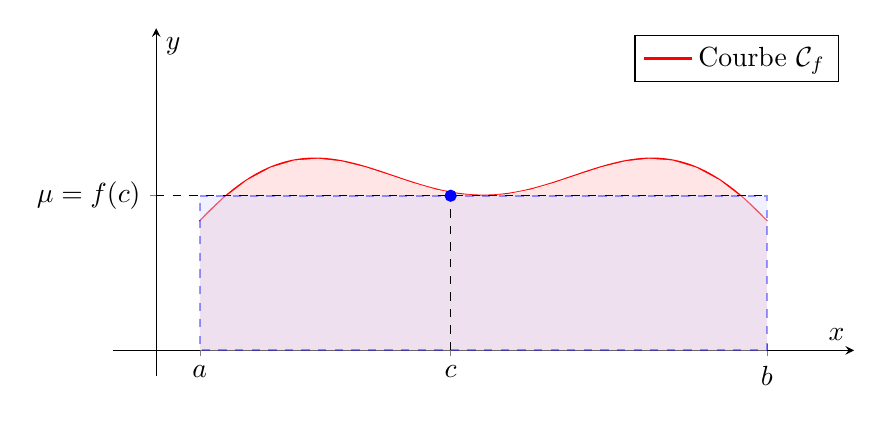
\begin{tikzpicture}
\begin{axis} [
    axis lines = middle,
    xlabel = $x$, ylabel = $y$,
    xmin = -0.2, xmax = 3.2,
    ymin = -0.2, ymax = 2.5,
    xtick = {0.2, 1.35, 2.8},
    xticklabels = {$a$, $c$, $b$},
    ytick = {1.2},
    yticklabels = {$\mu = f(c)$},
    width = 11cm, height = 6cm
]
% Courbe continue
\addplot [domain=0.2:2.8, samples=100, red, thick] {1.5 - 0.4*(x-1.5)^2 + 0.3*sin(180*x)};
\addlegendentry{Courbe $\mathcal{C}_f$}

% Aire sous la courbe f (hachurée ou colorée en rouge clair)
\addplot [domain=0.2:2.8, fill=red!10, draw=none] {1.5 - 0.4*(x-1.5)^2 + 0.3*sin(180*x)} \closedcycle;

% Rectangle de hauteur f(c) = 1.2 d'aire équivalente
\addplot [domain=0.2:2.8, fill=blue!15, opacity=0.4, draw=blue, dashed, thick] {1.2} \closedcycle;

% Point c, f(c)
\draw[dashed] (axis cs:1.35, 0) -- (axis cs:1.35, 1.2);
\draw[dashed] (axis cs:0, 1.2) -- (axis cs:2.8, 1.2);
\draw[blue, fill=blue] (axis cs:1.35, 1.2) circle (2pt);

\end{axis}
\end{tikzpicture}
\captionof{figure}{L'aire sous la courbe (en rouge clair) est rigoureusement égale à l'aire du rectangle bleu de hauteur $\mu = f(c)$.}
\end{center}


\section{Théorème fondamental de l'analyse}

Il s'agit du théorème clé établissant le pont définitif entre le calcul différentiel et l'intégration.

\subsection{La fonction "aire"}

\theorem{Théorème fondamental de l'analyse (TFA)}{}{true}{
    Soit $f : I \to \mathbb{R}$ une fonction \textbf{continue} sur un intervalle $I$ de $\mathbb{R}$. Soit $a \in I$ un point fixe.\\
    La fonction $F$ définie sur $I$ par :
    $$F(x) = \int_{a}^{x} f(t) \, dt$$
    est dérivable sur $I$, et sa dérivée vaut :
    $$\forall x \in I, \quad F'(x) = f(x)$$
    Autrement dit, $F$ est l'unique primitive de $f$ sur $I$ s'annulant au point $a$.
}
\vspace{.5cm}
\noindent\textbf{Preuve du TFA (cas $f$ croissante) :}\par\vspace{0.5em}
Soit $x \in I$ et $h > 0$ tel que $x+h \in I$. On forme le taux d'accroissement de $F$ entre $x$ et $x+h$ :
$$\frac{F(x+h) - F(x)}{h} = \frac{1}{h} \left( \int_{a}^{x+h} f(t)\,dt - \int_{a}^{x} f(t)\,dt \right) = \frac{1}{h} \int_{x}^{x+h} f(t)\,dt$$ (par la relation de Chasles).

Puisque $f$ est croissante sur $[x, x+h]$, on a pour tout $t \in [x, x+h]$ :
$$f(x) \le f(t) \le f(x+h)$$
En intégrant cette inégalité sur $[x, x+h]$, par croissance de l'intégrale, on obtient :
$$\int_{x}^{x+h} f(x) \, dt \le \int_{x}^{x+h} f(t) \, dt \le \int_{x}^{x+h} f(x+h) \, dt$$
$$h f(x) \le F(x+h) - F(x) \le h f(x+h)$$
Comme $h > 0$, en divisant par $h$ :
$$f(x) \le \frac{F(x+h) - F(x)}{h} \le f(x+h)$$
Puisque $f$ est continue en $x$, on a $\lim_{h \to 0^+} f(x+h) = f(x)$.\\
Par le théorème des gendarmes, on en déduit que :
$$\lim_{h \to 0^+} \frac{F(x+h) - F(x)}{h} = f(x)$$
Une démonstration analogue pour $h < 0$ prouve la limite à gauche. Ainsi, $F$ est dérivable au point $x$ et $F'(x) = f(x)$.\\

\subsection{Dérivée d'une intégrale à bornes variables}

Il est assez classique de devoir calculer la dérivée d'une fonction définie par une intégrale dont les bornes sont elles-mêmes des fonctions de la variable. Le théorème fondamental de l'analyse permet d'obtenir une formule explicite pour cette dérivée.

\theorem{Corollaire}{Généralisation aux bornes fonctionnelles}{false}{
    Soit $f : I \to \mathbb{R}$ une fonction continue sur un intervalle $I$.\\
    Soient $u, v : J \to I$ deux fonctions dérivables sur un intervalle $J$.\\
    Alors la fonction $g$ définie sur $J$ par :
    $$g(x) = \int_{u(x)}^{v(x)} f(t) \, dt$$
    est continue et dérivable sur $J$, et sa dérivée s'exprime par :
    $$\forall x \in J, \quad g'(x) = v'(x) f(v(x)) - u'(x) f(u(x))$$
}

\example{Soit $g(x) = \int_{x}^{2x} \frac{1}{1+t^2} \, dt$ définie sur $\mathbb{R}$. La fonction $f : t \mapsto \frac{1}{1+t^2}$ est continue sur $\mathbb{R}$. Les bornes $u(x) = x$ et $v(x) = 2x$ sont de classe $\mathcal{C}^1$ sur $\mathbb{R}$. Alors $g$ est dérivable sur $\mathbb{R}$ et :
$$g'(x) = 2 \times f(2x) - 1 \times f(x) = \frac{2}{1+4x^2} - \frac{1}{1+x^2}$$}

\section{Outils pour le calcul d'intégrales}

Il existe trois grandes techniques à maîtriser : l'intégration par parties, le changement de variable et l'application des formules de Taylor.

\subsection{Intégration par parties (IPP)}

\theorem{Proposition}{Formule d'Intégration par parties}{true}{
    Soient $u, v : [a, b] \to \mathbb{R}$ deux fonctions de classe $\mathcal{C}^1$ (dérivables et de dérivée continue) sur $[a, b]$. Alors :
    $$\int_{a}^{b} u(t) v'(t) \, dt = [u(t) v(t)]_a^b - \int_{a}^{b} u'(t) v(t) \, dt$$
}

\noindent\textbf{Preuve :}\\
\noindent\carreaux{8}

\example{Calculer l'intégrale $I = \int_{1}^{e} x \ln(x) \, dx$.\\
On pose :
$$\begin{cases} u(x) = \ln(x) & \implies u'(x) = \frac{1}{x} \\ v'(x) = x & \implies v(x) = \frac{x^2}{2} \end{cases}$$
Les fonctions $u$ et $v$ sont de classe $\mathcal{C}^1$ sur $[1, e]$. Par IPP, on a :
$$I = \left[ \frac{x^2}{2} \ln(x) \right]_1^e - \int_{1}^{e} \frac{x^2}{2} \times \frac{1}{x} \, dx = \left(\frac{e^2}{2} \times 1 - 0\right) - \frac{1}{2} \int_{1}^{e} x \, dx$$
$$I = \frac{e^2}{2} - \frac{1}{2} \left[ \frac{x^2}{2} \right]_1^e = \frac{e^2}{2} - \frac{1}{4}(e^2 - 1) = \frac{e^2 + 1}{4}$$}

\subsection{Changement de variable}

\theorem{Proposition}{Changement de variable}{true}{
    Soit $f : I \to \mathbb{R}$ une fonction continue sur un intervalle $I$.\\
    Soit $\varphi : [a, b] \to I$ une fonction de classe $\mathcal{C}^1$ sur le segment $[a, b]$. Alors :
    $$\int_{\varphi(a)}^{\varphi(b)} f(t) \, dt = \int_{a}^{b} f(\varphi(s)) \varphi'(s) \, ds$$
}

\method{Pratique du changement de variable}{
    Pour calculer l'intégrale $\int_{A}^{B} f(t) \, dt$ à l'aide de la transformation $t = \varphi(s)$ :
    \begin{enumerate}
        \item Remplacer l'élément différentiel : $dt = \varphi'(s) \, ds$.
        \item Convertir les bornes de l'intégration : si $t$ varie de $A$ à $B$, alors $s$ varie de $a = \varphi^{-1}(A)$ à $b = \varphi^{-1}(B)$ (si $\varphi$ est bijective).
        \item Substituer la variable dans l'intégrande : $f(t) \to f(\varphi(s))$.
    \end{enumerate}
}

\vspace{2cm}

\training{Calculer l'intégrale $J = \int_{0}^{1} \sqrt{1 - x^2} \, dx$ à l'aide du changement de variable $x = \sin(\theta)$ pour $\theta \in [0, \frac{\pi}{2}]$.} \par\vspace{0.5em}
\noindent\carreaux{10}

\subsection{Formule de Taylor avec reste intégral}

L'IPP permet de démontrer par récurrence ce théorème majeur, qui sert de pont entre l'approximation locale (les polynômes de Taylor) et l'analyse globale.

\theorem{Théorème}{Formule de Taylor avec reste intégral}{true}{
    Soit $f : I \to \mathbb{R}$ une fonction de classe $\mathcal{C}^{n+1}$ sur un intervalle $I$ de $\mathbb{R}$. Soient $a$ et $x$ deux points de $I$. Alors :
    $$f(x) = \sum_{k=0}^{n} \frac{f^{(k)}(a)}{k!} (x - a)^k + \int_{a}^{x} \frac{f^{(n+1)}(t)}{n!} (x - t)^n \, dt$$
}

\remark{La formule de Taylor est un outil formidable pour estimer précisément les erreurs d'approximation commises lorsqu'on remplace une fonction complexe par sa partie polynomiale.}

\section{Approximation par les sommes de Riemann}

Les sommes de Riemann constituent la méthode universelle d'approximation d'une intégrale par des rectangles de même largeur.

\definition{Soit $f : [a, b] \to \mathbb{R}$ une fonction continue.\\
Pour tout $n \in \mathbb{N}^*$, on appelle \textbf{somme de Riemann} (à gauche) associée à $f$ la quantité :
$$R_n(f) = \frac{b-a}{n} \sum_{k=0}^{n-1} f\left(a + k\frac{b-a}{n}\right)$$}

\theorem{Théorème}{Convergence des sommes de Riemann}{true}{
    Soit $f : [a, b] \to \mathbb{R}$ une fonction continue sur $[a, b]$. Alors la suite des sommes de Riemann converge vers l'intégrale de $f$ :
    $$\lim_{n \to +\infty} R_n(f) = \int_{a}^{b} f(t) \, dt$$
}

\method{Détermination de limites de suites de sommes}{
    Si une suite s'exprime sous la forme $S_n = \frac{1}{n} \sum_{k=1}^{n} g\left(\frac{k}{n}\right)$, on reconnaît une somme de Riemann régulière de la fonction $g$ sur $[0, 1]$. On a alors :
    $$\lim_{n \to +\infty} S_n = \int_{0}^{1} g(x) \, dx$$
}

\example{Déterminer la limite de la suite $U_n = \sum_{k=1}^{n} \frac{n}{n^2 + k^2}$.\\
On peut réécrire le terme général sous la forme :
$$U_n = \sum_{k=1}^{n} \frac{n}{n^2 \left(1 + \left(\frac{k}{n}\right)^2\right)} = \frac{1}{n} \sum_{k=1}^{n} \frac{1}{1 + \left(\frac{k}{n}\right)^2}$$
On identifie la somme de Riemann régulière associée à la fonction $g(x) = \frac{1}{1+x^2}$ sur $[0, 1]$.\\
La fonction $g$ étant continue sur $[0, 1]$, la suite converge, et sa limite vaut :
$$\lim_{n \to +\infty} U_n = \int_{0}^{1} \frac{1}{1+x^2} \, dx = [\arctan(x)]_0^1 = \arctan(1) - \arctan(0) = \frac{\pi}{4}$$}

\newpage
\tableofcontents
\section*{Crédits}
Ce cours reprend partiellement les travaux de M$^{\text{me}}$ \textsc{Yuen} et de M$^{\text{me}}$ \textsc{Mecherbet}, respectivement professeurs de mathématiques agrégé au lycée polyvalent Gustave Monod d'Enghien-les-Bains et maître de conférences à l'université Paris-Cité.\\

\end{document}